\documentclass{article}
\usepackage[x11names, rgb]{xcolor}
\usepackage[utf8]{inputenc}
\usepackage{tikz}
\usetikzlibrary{snakes,arrows,shapes}
\usepackage{amsmath}
%
%

%

%

\begin{document}
\pagestyle{empty}
%
%
%

\enlargethispage{100cm}
% Start of code
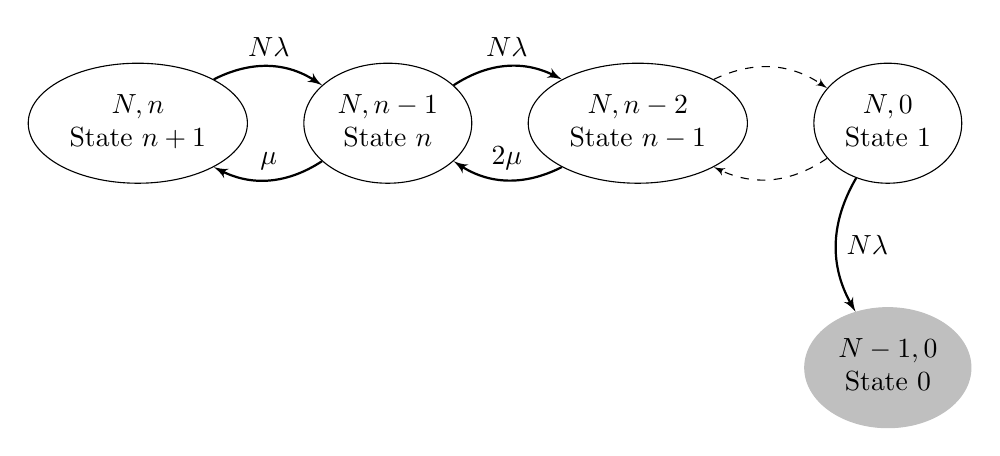
\begin{tikzpicture}[>=latex',line join=bevel,]
%%
\node (1) at (297bp,106bp) [draw,ellipse] {$\begin{matrix}N, 0 \\ \text{State }1 \end{matrix}$};
  \node (0) at (297bp,18bp) [draw=lightgray,fill=lightgray,ellipse] {$\begin{matrix}N-1, 0 \\ \text{State }0 \end{matrix}$};
  \node (3) at (117bp,106bp) [draw,ellipse] {$\begin{matrix}N, n-1 \\ \text{State }n \end{matrix}$};
  \node (2) at (207bp,106bp) [draw,ellipse] {$\begin{matrix}N, n-2 \\ \text{State }n-1 \end{matrix}$};
  \node (4) at (27bp,106bp) [draw,ellipse] {$\begin{matrix}N, n \\ \text{State }n+1 \end{matrix}$};
  \draw [->,thick] (1) to[bend right] node[right] {$N\lambda$} (0);
  \draw [->,thick] (2) to[bend left] node[above] {$2\mu$} (3);
  \draw [->,dashed] (2) to[bend left] node[above] { } (1);
  \draw [->,thick] (3) to[bend left] node[above] {$N\lambda$} (2);
  \draw [->,dashed] (1) to[bend left] node[above] { } (2);
  \draw [->,thick] (4) to[bend left] node[above] {$N\lambda$} (3);
  \draw [->,thick] (3) to[bend left] node[above] {$\mu$} (4);
%
\end{tikzpicture}
% End of code

%
\end{document}
%



